\documentclass[letterpaper,twocolumn,10pt]{article}
\usepackage[margin=0.75in]{geometry}

\usepackage{graphicx}
\newcommand{\vB}{\mbox{$\bf v$}}
\newcommand{\xB}{\mbox{$\bf x$}}
\newcommand{\yB}{\mbox{$\bf y$}}
\newcommand{\JB}{\mbox{$\bf J$}}
\newcommand{\RB}{\mbox{$\bf R$}}
\newcommand{\WB}{\mbox{$\bf W$}}
\newcommand{\PB}{\mbox{$\bf P$}}
\newcommand{\MB}{\mbox{$\bf M$}}
\newcommand{\IB}{\mbox{$\bf I$}}
%\newcommand{\SG}{\mbox{$\mathbf \Sigma$}}
%\newcommand{\sG}{\mbox{$\mathbf \sigma$}}
\newcommand{\SG}{\mbox{$\bf \Sigma$}}
\newcommand{\sG}{\mbox{$\bf \sigma$}}
\newcommand{\etal}{{\em et al}}
\begin{document}

\title{\bf 
Simple FEMs aren't as good as we thought: \\
  experiences developing EIDORS v3.3%
}

\author{Andy Adler$^{1}$,
        Andrea Borsic$^{2}$,
        Nick Polydorides$^{3}$,
        William R B Lionheart$^{4}$}
\date{}
\maketitle

%\begin{abstract}
\section*{Abstract}
{\small
This paper covers three topics. First, we announce
EIDORS version 3.3, and clarify the new features and
changes to the software.
Next, we review the use of dual models in EIT, and
architecture to support their use in EIDORS.
Last,
we discuss accuracy limitations to the single-order
tetrahedral finite element models that are used
in much EIT research. Specifically, the accuracy
of simulated voltages is explored as a function
of mesh density and electrode refinement.
A conductive object was simulated moving in a 
circular tank, using adaptive mesh refinement
around the object. Images were reconstructed
using difference EIT and compared to those from
a saline tank phantom.
FEM accuracy may be partially addressed using
dual model solvers, for which EIDORS v3.3
provides support.
Briefly, the new version also includes:
1) interfaces to FEM generation (distmesh, netgen) and 
  dual model solvers
2) new algorithms (total variation, electrode movement solver,
  temporal solvers) 
3) a data repository with several contributed models, clinical
   and experimental data sets
4) faster algorithms with better caching, and
5) improved graphics and extensive tutorials
}
%\end{abstract}
\\

{\small
\noindent
$^1$Systems and Computer Engineering, Carleton University, Ottawa, Canada
$^2$Thayer School of Engineering, Dartmouth College, Hannover, NH, USA
$^3$School of Engineering, Massachusetts Institute of Technology, Boston, USA
$^4$School of Mathematics, University of Manchester, UK
}

\section{Introduction}

We address three issues in this paper. Perhaps, the most surprising
result is the third, that 
\begin{quote}
   simple (tetrahedral first-order) finite element models (FEMs)
      aren't as good as we thought.
\end{quote}
Models with up to 10,000 elements (2D) or 1,000,000 elements
(3D) are not able to reproduce the accuracy of tank phantom
measurements.

First, we announce
release version 3.3 of EIDORS (Electrical Impedance Tomography and
 Diffuse Optical Tomography Reconstruction Software),
and report on the new features and their use. One important
addition is the repository for contributed experimental 
(physiological and phantom) and
clinical data and FEM models, which we document here.

Next, we review the formulation of image reconstruction based
on dual models, in which a refined fine FEM (finite element
model) is used for the forward model, and a
coarse mesh (not necessarily based on FEM) is used of image
reconstruction. Dual models have been used in many EIT algorithms,
and we review their use, and provide an algorithmic framework
to describe their application. EIDORS v3.3 provides an
architecture to support general variations of dual models,
which we describe.

Third, since dual models are designed to allow use of large
FEMs for forward modelling, we explore the accuracy of the
first order tetrahedral models that are most commonly used
in EIT research. Our results indicate that these models
perform surprisingly poorly, and only slowly approximate
the underlying phantom as the number of elements grows.
This effect is particularly severe in 3D FEM models, because
the number of elements required to achieve a given element
size is larger by a power of $\frac{3}{2}$.
In the final version of this paper, we will provide a
test method to identify the appropriate size
of FEM required for a specified accuracy.
 

\section{EIDORS version 3.3}

EIDORS (Electrical Impedance Tomography and Diffuse Optical
 Tomography Reconstruction Software) is an open source
suite of software for reconstruction of images in soft 
field tomography modalities. The earliest version was made
available in 1999 and provided support for 2D EIT (Vauhkonen).
Subsequently, support for 3D EIT was provided (Polydorides) in 
2000. In 2005, EIDORS was refactored to allow ``pluggability''
-- easy incorporation of contributed algorithms and 
functionality -- as part of EIDORS version 3 (while the
previous releases were renamed v1 and v2, respectively). 
Version $3.0$ was released in 2005, v3.1 in 2006 (and described
in Adler and Lionheart, 2006), v3.2 in 2007, and v3.3
(described in this paper). Many new features have been added;
in terms of lines of code, v2.0 has 3715, v3.0 has 10685
and v3.3 has 27774 (with another 5940 in tutorials).

The following high-level new features are part of EIDORS v3.3:

\newcounter{Ictr}
\begin{list}{\bf \arabic{section}.\arabic{Ictr}}
  {\leftmargin=0.0em \itemindent=2.0em
%   \topsep= 0.0\baselineskip
%   \itemsep=-0.0em
    \listparindent=1.0em \parsep=-0.0em
    \usecounter{Ictr}}
\item {\bf interfaces to FEM generation}

Interfaces to Netgen (Sch\"oberl, 1997), Distmesh (Persson and Strang, 2004)

\item {\bf support for dual model solvers}

\item {\bf new algorithms}
 (total variation, electrode movement solver,
  temporal solvers)

\item {\bf data repository}
 with several contributed models, clinical
   and experimental data sets

\item {\bf faster algorithms}
   PDIPM, Jacobian, with better caching

\item {\bf improved graphics and extensive tutorials}

\end{list}

\section{Dual Model solvers}

\begin{figure}[tbh]
\begin{center}
 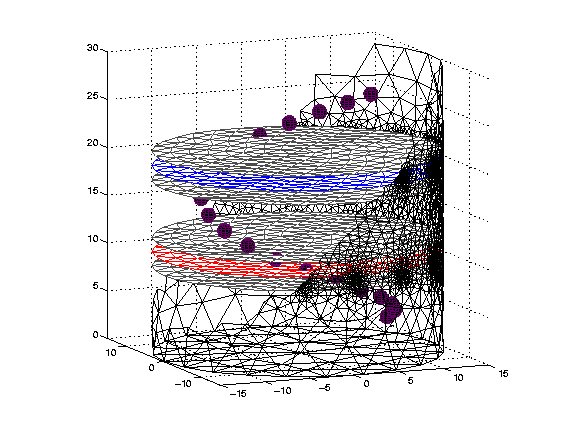
\includegraphics[width= 0.45\textwidth]{../../tutorial/dual_model/centre_slice02a.png}
\caption{ \label{fig:dual_model}
\small
Netgen model of a 2�16 electrode tank. The positions of the simulated
conductive target moving in a helical path are shown in purple. The
3D fine model is shown (cropped). The upper (blue) and lower (red)
layers corresponding to the geometry of the coarse model are shown. The
z direction limits of the coarse model are shown in grey.
}
\end{center}
\end{figure}

\begin{figure}[tbh]
\begin{center}
 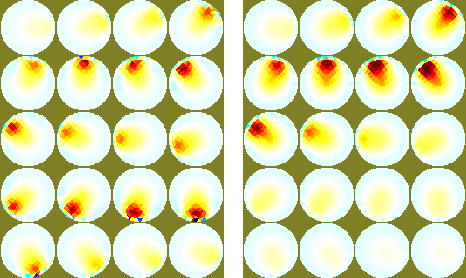
\includegraphics[width= 0.45\textwidth]{figs/centre_slice04a_crop.png}
\caption{ \label{fig:dual_model_reconst}
\small
Reconstructed images of a target moving in a helical pattern using
difference reconstruction models.
{\em Left} reconstruction model with  $z_{depth}=\infty$
{\em Right} reconstruction model with $z_{depth}= 0.1\times \mbox{scale}$
at lower position in Fig. \ref{fig:dual_model}
}
\end{center}
\end{figure}

A dual reconstruction model uses a fine finite element
model (FEM) to implement the forward solution (voltages
at electrodes), and a coarse mesh for the inverse
solution. For example, a dual model may be used to 
represent the conductivity change in a layer
of a 3D plane (ie. Fig. \ref{fig:dual_model}).
Given a forward model, $F$,
which calculates a voltage measurement vector, $\vB$, from
a forward (fine) model conductivity element vector, $\sG_f$, we
have $\vB = F( \sG_f )$. The reconstruction (coarse)
model is defined on square elements $\sG_r$ related by
a coarse to fine projection matrix $\PB$, where $\sG_f = \PB \sG_r$.

This is implemented in EIDORS as follows. For each
inverse model, represented as part of the {\tt inv\_model}
structure (Fig \ref{fig:invmdl}),
there are two {\tt fwd\_model} structures:
1) the refined forward model {\tt fwd\_model}, and
2) the reconstruction model {\tt rec\_model}. 
Within each forward model structure is a matrix field
{\tt coarse2fine} which is a sparse encoding of $\PB$.
Each element $[\PB]_{i,j}$ represents the fraction of
fine element $i$ enclosed within coarse element $j$.

TODO: Discuss fast calculation of coarse2fine.

The need for a matrix $\PB$ on the {\tt rec\_model} is
due to the limits of the first order FEM representation.
If the regions in the reconstruction model are not
triangular, then each region is constructed from triangular
regions and the parametrization represented in $\PB$.

\begin{figure}[tbh]
\begin{center}
 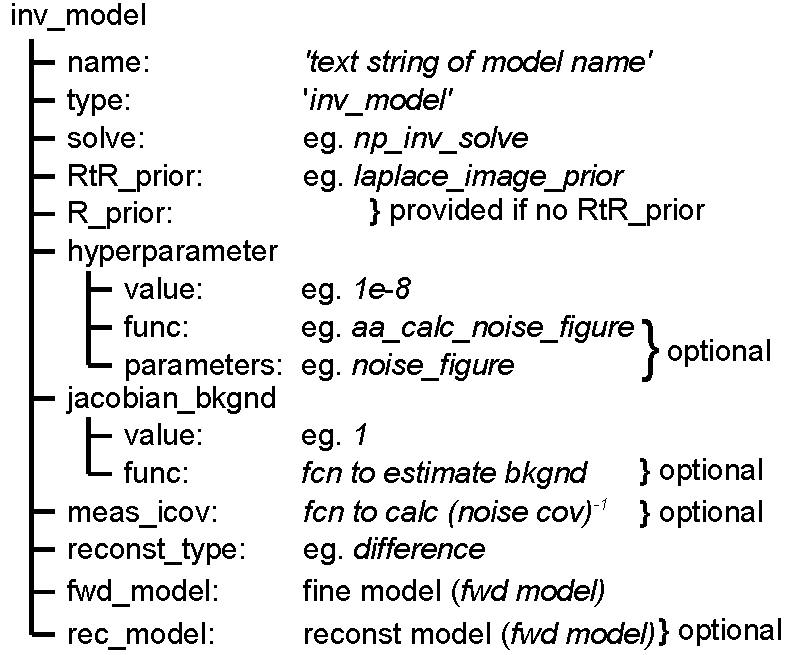
\includegraphics[width= 0.40\textwidth]{figs/inv_model.png}
\caption{ \label{fig:invmdl}
\small
Layout of the EIDORS {\tt inv\_model} object
}
\end{center}
\end{figure}

Dual meshes may be used in several applications:
\begin{list}{$\circ$} %{\textbullet}
  {\leftmargin=1.0em \itemindent=-0.0em
    \topsep=0.0\baselineskip
    \itemsep=-0.4\baselineskip}
\item
   corresponding meshes (coarse elements completely contain fine ones)
\item
   elem to node (nodal solvers)
\item
   $2\frac{1}{2}$D solvers, in which the $z$-dimension of the
     3D fine model is projected onto the coarse.
\item
   constraining parameter choices (ie. having one parameter
      for out of plane conductivity to prevent the system from
      "pushing" artefacts there.)
\item
   solving to a rasterized grid (as in GREIT)
\end{list}


Dual meshes have been used by many EIT groups
\\
- Oxford Brookes used an interpolation method on two meshes since the early code in the Fortran code Recon started by Lionheart and continued by Kevin Paulson at Brookes. The approach used a mesh correspondence array. 
\\
- Later on the Dartmouth group also used the idea; paper by the
   similarly named Keith Paulsen (ref).
\\
- Marko Vauhkonen use two meshes in the original 2D EIDORS.
\\
- UCL optimal tomography group uses it for TOAST.

\section{FEM accuracy}

\begin{figure}[tbh]
\begin{center}
 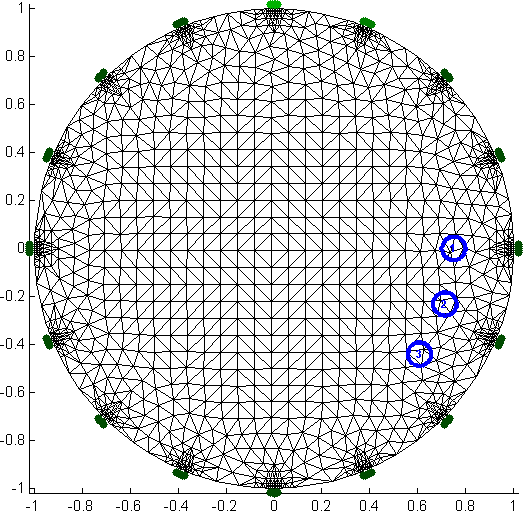
\includegraphics[width= 0.24\textwidth]{figs/fig1a.png}
 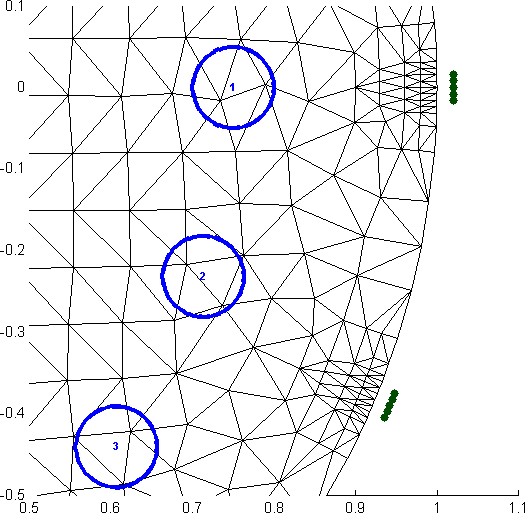
\includegraphics[width= 0.24\textwidth]{figs/fig1b.png}
\caption{ \label{fig:fem1}
\small
Simulation FEM and simulated target positions in blue
{\em Left} full scale mesh.
{\em Right} mesh magnified near target positions 
}
\end{center}
\end{figure}

\begin{figure}[tbh]
\begin{center}
 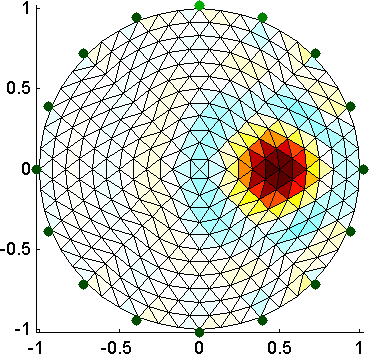
\includegraphics[width= 0.15\textwidth]{figs/fig2a.png}
 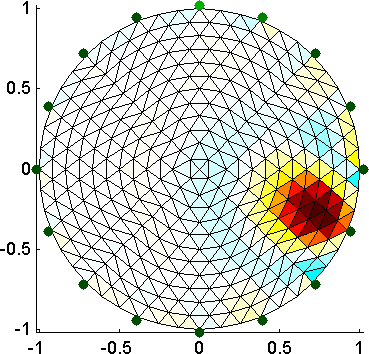
\includegraphics[width= 0.15\textwidth]{figs/fig2b.png}
 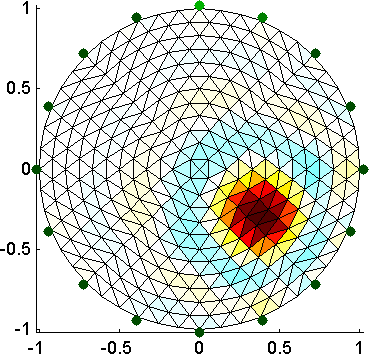
\includegraphics[width= 0.15\textwidth]{figs/fig2c.png}
\caption{ \label{fig:fem1_images}
\small
Images reconstructed of targets simulated from
interpolated shapes in Fig. \ref{fig:fem1}, from
left to right, targets 1 to 3.
}
\end{center}
\end{figure}

Finite Element Model (FEM) accuracy is normally considered
from the point of view of voltage errors between FEM and
physical phantom. While this is correct, any errors may be explained
by small details in the phantom which are not considered
in the model. Here we consider FEM accuracy from the
approach of looking at small changes in the model and their
consequences on time difference EIT images.

The easiest (and most common) way to simulate a moving target
in a medium is to use a single FEM to select and then interpolate
which elements are part of that target. Fig. \ref{fig:fem1}
shows two 2372 element FEM created by distmesh, with mesh
refinement near the electrodes. Sixteen electrodes are
simulated using a Sheffield-type adjacent stimulation and
measurement. For each simulated target position (blue), the
fraction of each element filled by the target is calculated
and the conductivity change is scaled by this fraction.

Images are reconstructed of the three target positions
in Fig. \ref{fig:fem1_images} using a one-step regularized
GN image reconstruction. There is no change to
the underlying FEM, and thus no noise in the images.

However, the best way to simulate a moving target is
create a target region within the FEM and to remesh around
it. This means that the mesh changes between each
target position, not only near the target, but throughout
the FEM due to the propagation of changes in triangularization.

\begin{figure}[tbh]
\begin{center}
 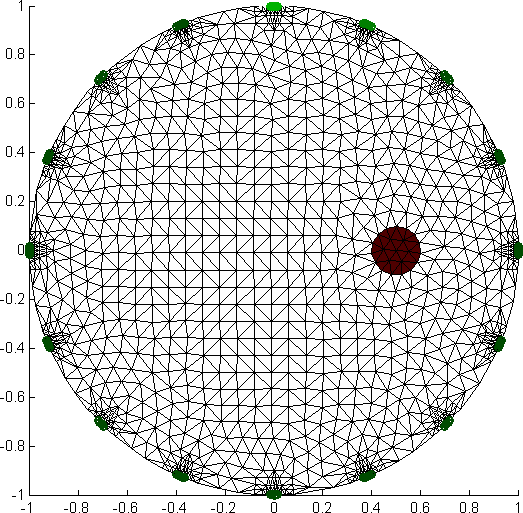
\includegraphics[width= 0.20\textwidth]{figs/fig3a-2372e.png}
 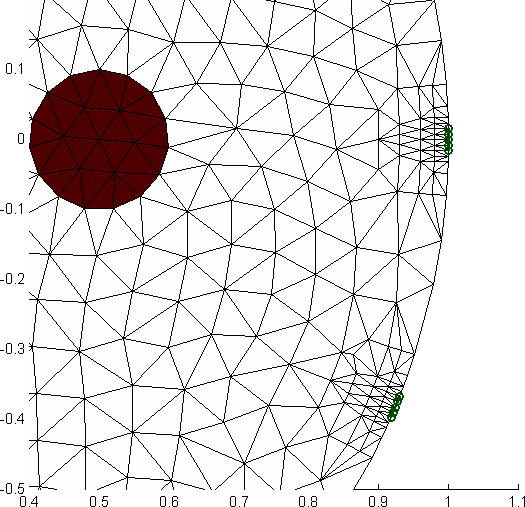
\includegraphics[width= 0.20\textwidth]{figs/fig3b-2372e.png}
 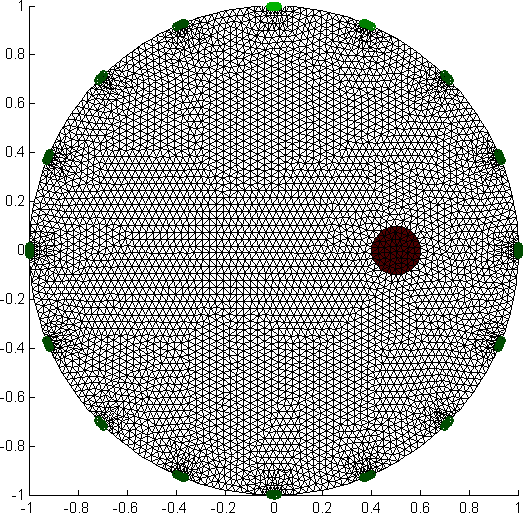
\includegraphics[width= 0.20\textwidth]{figs/fig3a-8909e.png}
 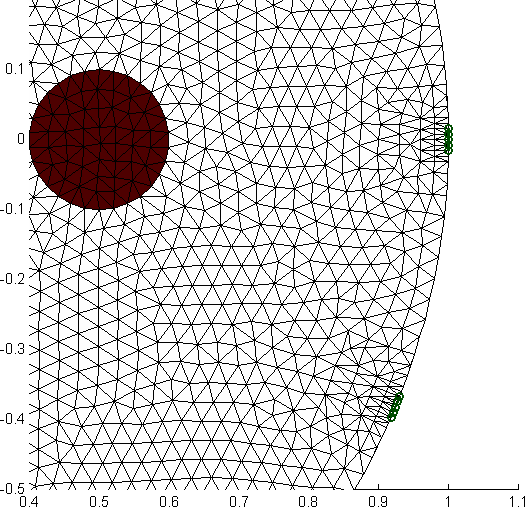
\includegraphics[width= 0.20\textwidth]{figs/fig3b-8909e.png}
\caption{ \label{fig:fem2}
\small
Simulation FEM and simulated target positions in blue
{\em Left} full scale mesh.
{\em Right} mesh magnified near target positions 
{\em Top} FEM with 2372 elements,
{\em Bottom} FEM with 8909 elements,
}
\end{center}
\end{figure}

Using distmesh, FEMs were created of a homogeneous phantom
(like that of Fig. \ref{fig:fem1}), and of three phantoms
with inset targets at corresponding to the positions in
that figure.  Fig. \ref{fig:fem2} shows the mesh at the
first target position. Three different levels of mesh
refinement are shown.

Based on these simulations, we reconstruct images
using a simple 576 element mesh with point electrodes
(Fig. \ref{fig:fem2_images}. In the coarse (2372 element)
and to a lesser extent in the refined (8909 element) 
mesh, there are artefacts, mostly near the electrodes, which
dramatically disturb the image clarity.

\begin{figure}[tbh]
\begin{center}
 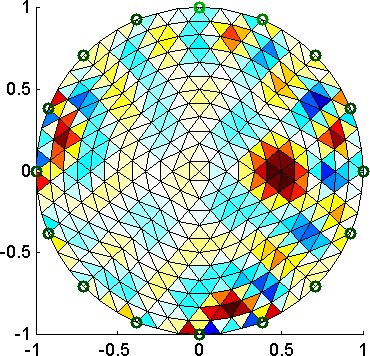
\includegraphics[width= 0.15\textwidth]{figs/fig4a-2372e.png}
 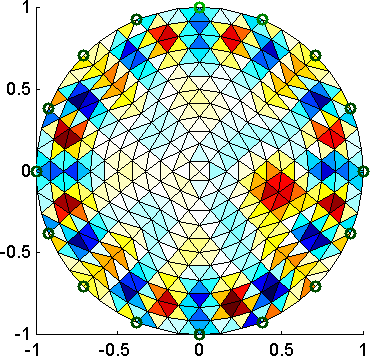
\includegraphics[width= 0.15\textwidth]{figs/fig4b-2372e.png}
 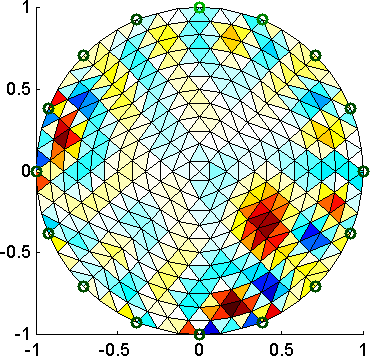
\includegraphics[width= 0.15\textwidth]{figs/fig4c-2372e.png}
 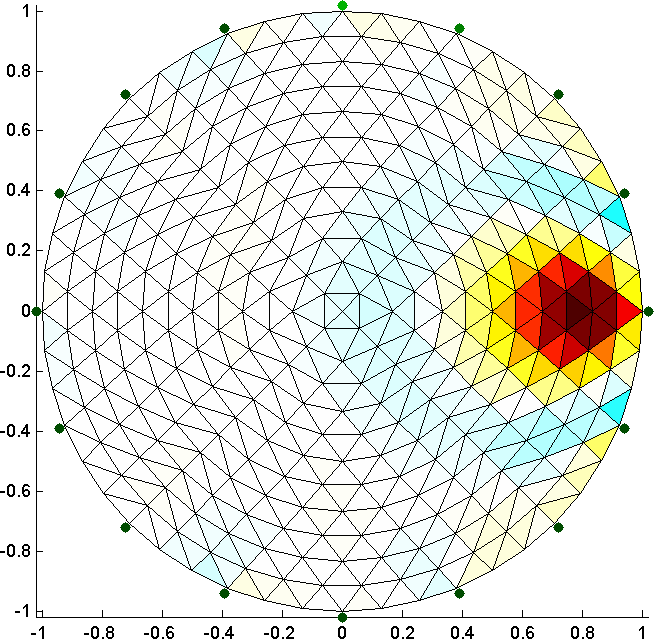
\includegraphics[width= 0.15\textwidth]{figs/fig4a-8909e.png}
 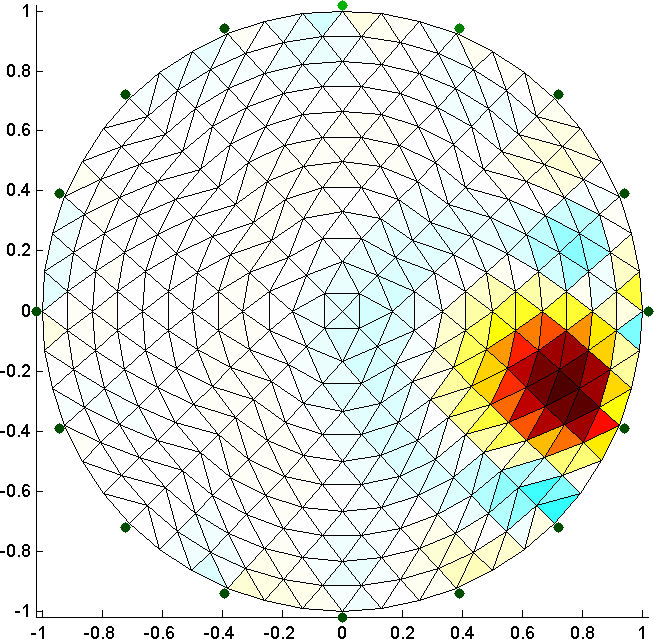
\includegraphics[width= 0.15\textwidth]{figs/fig4b-8909e.png}
 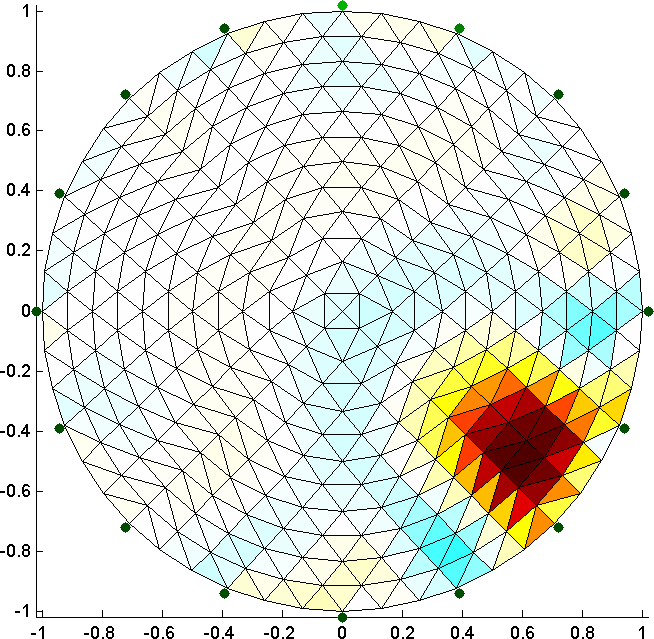
\includegraphics[width= 0.15\textwidth]{figs/fig4c-8909e.png}
\caption{ \label{fig:fem2_images}
\small
Images reconstructed of targets simulated from
interpolated shapes in Fig. \ref{fig:fem2}, from
left to right, targets 1 to 3.
{\em Top} FEM with 2372 elements,
{\em Bottom} FEM with 8909 elements,
}
\end{center}
\end{figure}

\begin{figure}[tbh]
\begin{center}
 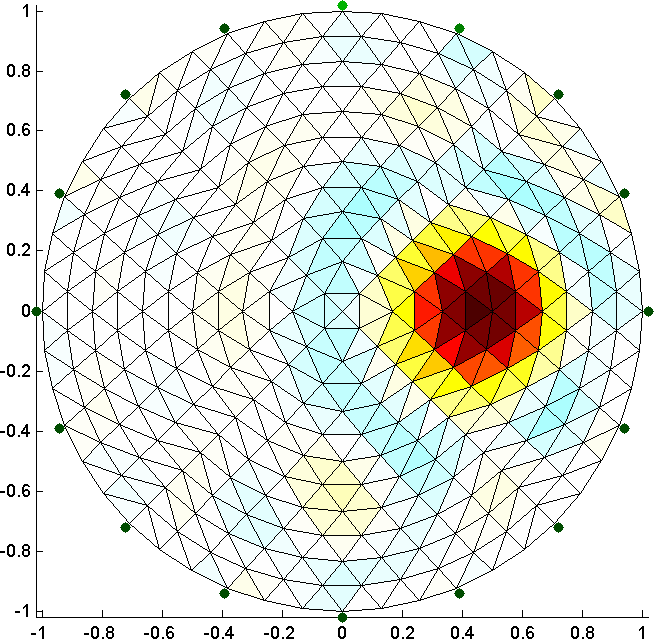
\includegraphics[width= 0.15\textwidth]{figs/fig5a.png}
 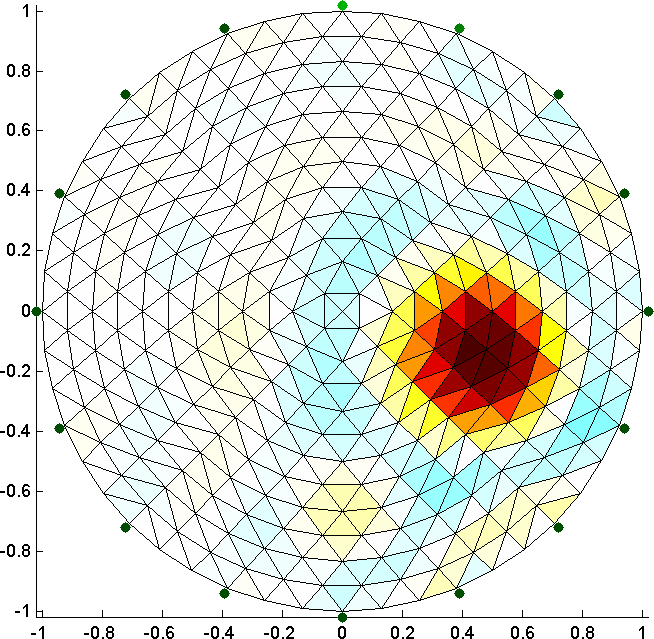
\includegraphics[width= 0.15\textwidth]{figs/fig5b.png}
 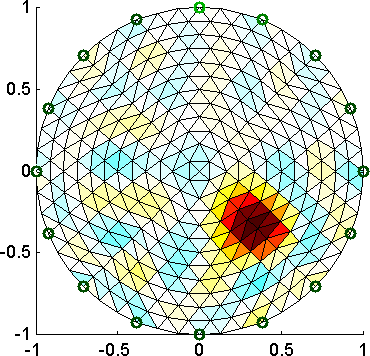
\includegraphics[width= 0.15\textwidth]{figs/fig5c.png}
\caption{ \label{fig:iirc_data}
\small
Images reconstructed of a target in a saline tank
with the same reconstruction parameters.
}
\end{center}
\end{figure}

To compare with these images, a sequence of EIT
data were gathered with a 16 electrode system from
the IIRC from Kyung Hee University, Korea. A saline
filled tank was used and a small non-conductive target
was slowly rotated around the tank. Frames of data
corresponding to the simulated positions are shown.
Images are reconstructed from these data using the
same reconstruction parameters and shown in
 Fig. \ref{fig:iirc_data}

\begin{figure}[tbh]
\begin{center}
 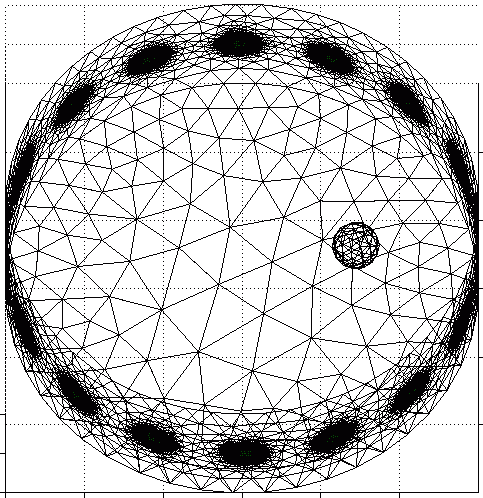
\includegraphics[width= 0.23\textwidth]{figs/fig6a.png}
 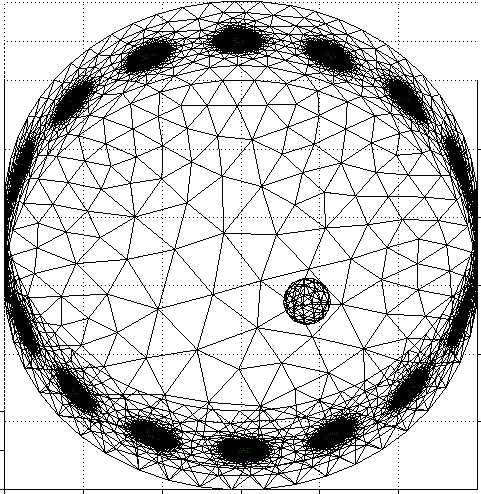
\includegraphics[width= 0.23\textwidth]{figs/fig6b.png}
\caption{ \label{fig:netgen_3D}
\small
3D models of a moving ball in a 16 electrode tank
with approximately $25,000$ elements,  using Netgen.
To simplify
the figure, only outer boundary elements are shown, including
the non-conductive ball in the centre.
}
\end{center}
\end{figure}


The same effect can be seen in 3D FEM, and is even
more significant because it the number of elements
required is larger because of the additional
dimension. We built a several 3D FEMs from
25,000 to 500,000 elements FEM using
netgen to study the effect.
Fig. \ref{fig:netgen_3D} shows the 25,000 element
mesh.


\section{Discussion}

This paper covers three topics: 1) announcement of
EIDORS version 3.3, and clarification of the new features and
changes to the software;
2) review of the use of dual models in EIT, and
the architecture to support their use in EIDORS;
and
3) discussion of accuracy limitations to the single-order
tetrahedral finite element models that are used
in much EIT research.
...

\end{document}

